\documentclass[paper=letter, onecolum, fontsize=12pt]{article}
\usepackage[english,activeacute]{babel}
\usepackage{amsmath,amsfonts,amsthm}
\usepackage[utf8]{inputenc}
\usepackage{float}
\usepackage{babel}
\usepackage{lipsum}
\usepackage{blindtext}
\usepackage{graphicx}
\usepackage{hyperref}
\usepackage{braket}
\usepackage{caption}
\usepackage{subcaption}
\usepackage[sc]{mathpazo}
\usepackage[T1]{fontenc}
\linespread{1,04}
\usepackage{microtype} 
%\usepackage[hmarginratio=1:1,top=32mm,columnsep=10pt]{geometry} 
\usepackage[left=1.5cm,top=2.5cm,right=1.5cm,bottom=2.5cm]{geometry}
\usepackage{multicol} 
\usepackage{booktabs}
\usepackage{ mathrsfs }
\usepackage{float} 
\usepackage{hyperref} 
\usepackage{lettrine} 
\usepackage{paralist} 
\usepackage{abstract} 
\usepackage{pstricks}
\usepackage{cancel}% Contain the most of the PSTricks commands.
\usepackage{pst-all}	        % Contain all the PSTricks commands.
\usepackage{pst-node}	% to define nodes and conexions between themselves.
\usepackage{pst-circ}         % to make electric circuits.
\renewcommand{\abstractnamefont}{\normalfont\bfseries}
\renewcommand{\abstracttextfont}{\normalfont\small\itshape} 
\usepackage{titlesec} 
\newcommand{\dbar}{\mathchar'26\mkern-12mu d}
\renewcommand\thesection{\Roman{section}} 
\renewcommand\thesubsection{\Roman{subsection}} 
\titleformat{\section}[block]{\large\scshape\centering}{\thesection.}{1em}{} 
\titleformat{\subsection}[block]{\large}{\thesubsection.}{1em}{} 
\newcommand{\horrule}[1]{\rule{\linewidth}{#1}} 
\usepackage{fancyhdr} 
\pagestyle{fancy} 
\fancyhead[C]{ $\bullet$ } 

%----------------------------------------------------------------------------------------
%       TITLE SECTION
%----------------------------------------------------------------------------------------
\title{\vspace{-10mm}\fontsize{21pt}{10pt}\selectfont
\textbf{KcsA embedded in POPC membrane: Stability Analysis}} % Article title
\author{
\large
{\textsc{Julietta Sophia Mendivelso\footnote{jsmendivelsor@unal.edu.co}}}
%\thanks{A thank you or further information}\\ % Your name
%\normalsize \href{mailto:marco.torres.810@gmail.com}{marco.torres.810@gmail.com}\\[2mm] % Your email address
}
\date{Computational Methods\\
Serrapilheira/ICTP-SAIFR Training Program in Quantitative Biology and Ecology}


%----------------------------------------------------------------------------------------
%\twocolumn
\begin{document}
\maketitle
\vspace{-10mm}
\section{Introduction}

\hspace{4mm} The KcsA (K channel of streptomyces A) membrane protein is an archetypal potassium channel that has been extensively studied in ion channel research. It is a prokaryotic potassium channel made of four identical subunits forming a tetramer, possesses two transmembrane segments \cite{schrempf_prokaryotic_1995} (Figure \ref{kcsa}) and a highly selective pore region that permits selective conduction of potassium ions at nearly bulk \cite{aksimentiev_tutorial_nodate}.\\

\begin{figure}[H]
    \centering
    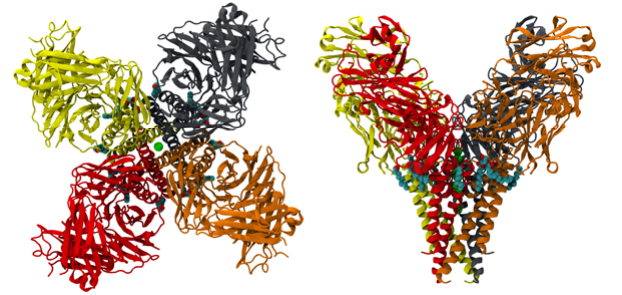
\includegraphics[width=0.7\textwidth]{kcsa_tetra.png}
    \caption{Top and side views of the KcsA tetramer. \cite{aksimentiev_tutorial_nodate}}
    \label{kcsa}
\end{figure}

KcsA was the first potassium ion channel to be characterized using x-ray crystallography \cite{doyle1998structure}. It belongs to a family of channels found in almost all organisms and its channels have diverse functions and have been implicated in osmotic regulation and neuronal signaling \cite{roux_ion_2005}. Since KcsA is a transmembrane protein, which means that spans the entirety of the cell membrane, studying its behavior, response and effects when interacting with a lipid membrane results relevant to the understanding of important structural and mechanistic properties of the $K^+$ channel function, and its elucidated structure underlies computational modeling of channel dynamics for both prokaryotic and eukaryotic species \cite{zhou_kcsa_2001}.\\

Here, full length protein structure for KcsA was embedded in atomistic lipid bilayer of POPC (1-palmitoyl-2-oleoyl-sn-glycero-3-phosphocholine), and solvated under physiological conditions (150mM NaCl). Atomistic molecular dynamics (MD) simulations were conducted to determine the structural integrity of the structure over simulations. The analysis of the structural integrity of KcsA by means of root mean square deviations and root mean square fluctuations in the simulations exposed the overall stability of the protein. Furthermore, the moving average analysis conducted over the pressure during the simulations reflected the stability of the entire KcsA-POPC system.

\section{Methods}

\subsection{Data}
\hspace{4mm} The tertiary structure of KcsA was obtained using X-ray crystallography \cite{doyle1998structure}. The data was deposited as a \textbf{.pdb} file in the \textit{Protein Data Bank} and its freely accessible on the Internet \cite{bank_rcsb_nodate}.\\

The .pdb file contains a monomer of the KcsA protein \textit{(1K4C.pdb)} and everything else solved from the crystal structure. The tetramer was built and embedded in the POPC membrane following the steps on the Membrane Protein Tutorial \cite{aksimentiev_tutorial_nodate}, using the \textbf{VMD} software \cite{humphrey_vmd_1996}.\\

The simulations for minimization, equilibration and production runs of the membrane-protein system were performed using \textbf{NAMD}, a parallel molecular dynamics code designed for high-performance simulation of large biomolecular systems \cite{phillips_namd_2020}.\\

The file with the pressure values during the simulation was obtained using the \textit{NAMD plot plugin} for VMD \cite{noauthor_namd_nodate}.

\subsection{RMSD analysis}

\hspace{4mm}The Root Mean Square Deviation (RMSD) of atomic positions is the measure of the average distance between the atoms (usually the backbone atoms) of superimposed proteins \cite{kufareva_methods_2011}. It is defined as 
\begin{equation*}
    RMSD=\sqrt{\frac{1}{N}\sum_i^N \delta_i^2},
\end{equation*}

Where $\delta_i$ is the distance between atom $i$ and either a reference structure or the mean position of the $N$ equivalent atoms.\\

The RMSD of the protein backbone gives an idea of the stability of the protein. If the RMSD is still increasing at the end of the simulation, the protein is still searching for a lower energy state, and thus is not yet stable.

\subsection{RMSF analysis}

\hspace{4mm}The Root Mean Square Fluctuation (RMSF) measures the average deviation of an atom over time from a reference position (typically the time-averaged position of the particle). Thus, RMSF analyzes the portions of structure that are fluctuating from their mean structure the most \cite{kufareva_methods_2011}. It is typically plotted vs. residue number, and can indicate structurally which amino acids in a protein contribute the most to a molecular motion. A small value of the RMSF indicates that the protein is conformationally stable.

\subsection{Moving average in pressure analysis}

\hspace{4mm} During a MD simulation, achievement of equilibrium is judged by how well velocities, pressure, etc. are distributed in the system over a given amount of time. \textit{NAMD} calculates system pressure based on
the forces between atoms and their kinetic energies, and it usually presents many fluctuations along the simulation. Considering this, a good way to determine the stability of the system in the simulation is calculating the moving average, which is commonly used with time series to smooth out the short-term fluctuations and highlight the longer-term trend of the data.

\section{Results}

\hspace{4mm}The plot for the RMSD along the trajectory (Figure \ref{rmsd}) showed a high increasing during the first steps of the simulation. However, in the next steps the RMSD showed small fluctuations and a slow increasing of its value. This result leds to conclude that KcsA is conformationally stable.
\begin{figure}[H]
    \centering
    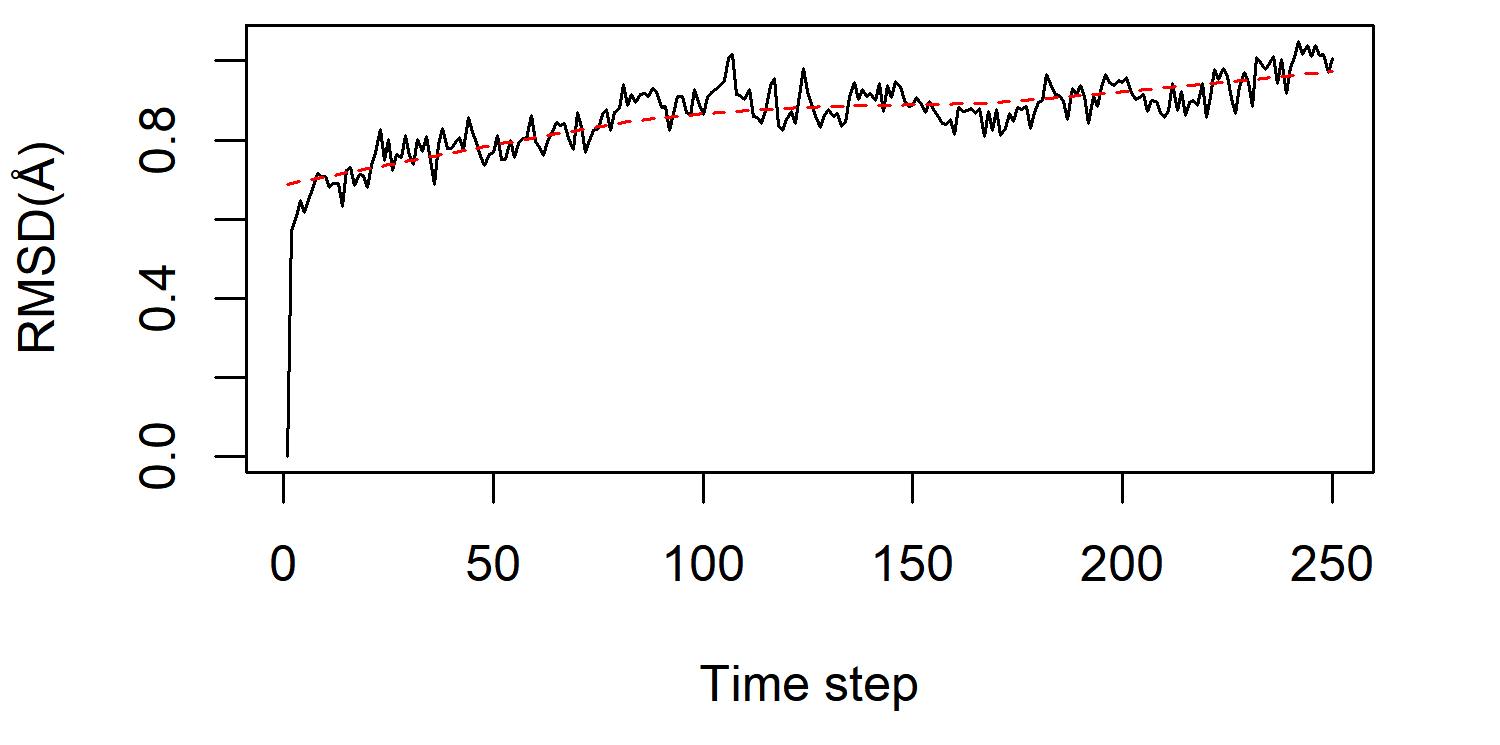
\includegraphics[width=0.7\textwidth]{rmsd.png}
    \caption{RMSD vs. Time step. One time step is equivalent to 2000 fs. The red line represents the LOWESS smoothing of the RMSD.}
    \label{rmsd}
\end{figure}
\vspace{-3mm}
 The plot for the RMSF showed small fluctuations over the simulation (Figure \ref{rmsf}). Even when some residues showed a higher fluctuation, this remains below $1.5 \AA$, which means that KcsA is stable when is embedded in the POPC membrane.
\begin{figure}[H]
    \centering
    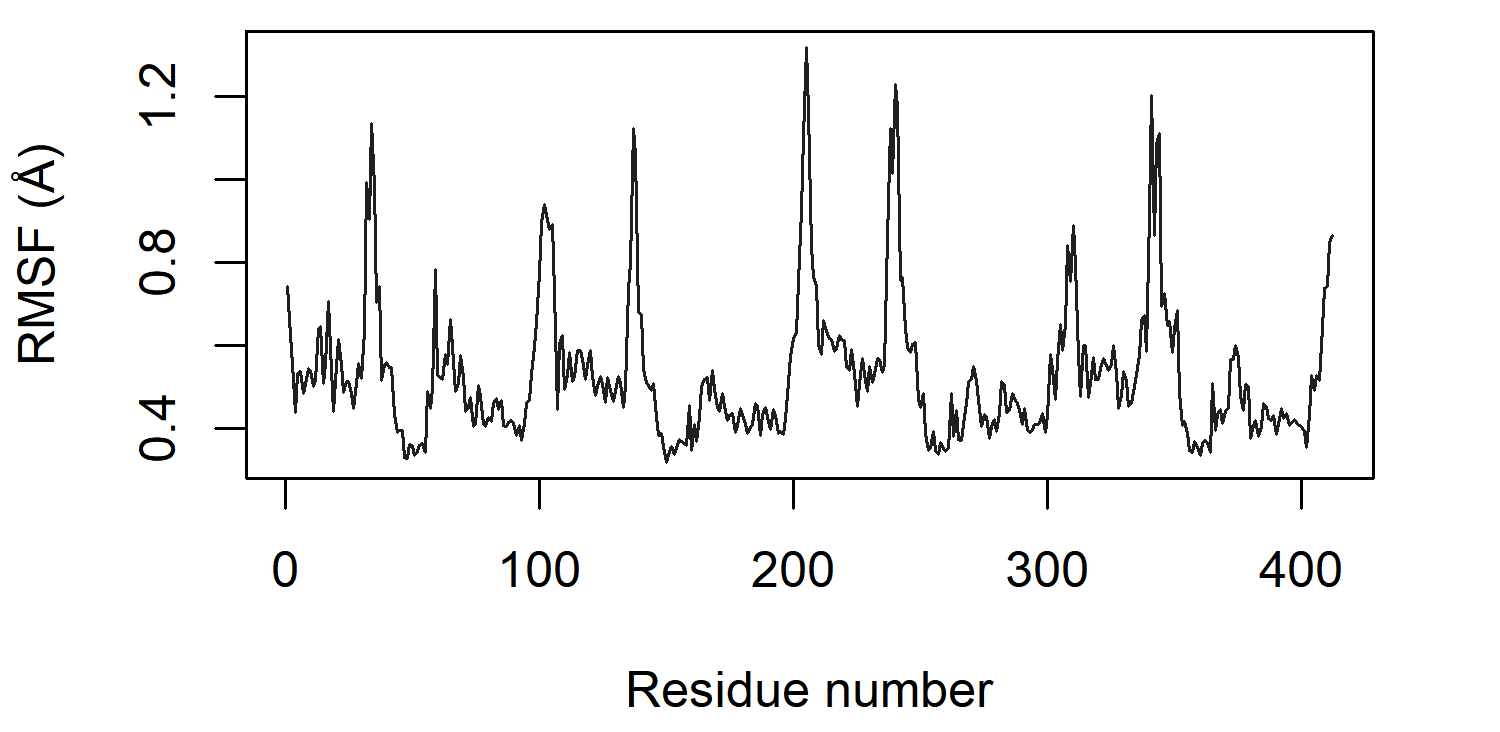
\includegraphics[width=0.7\textwidth]{rmsf.png}
    \caption{RMSF vs. Residue number.}
    \label{rmsf}
\end{figure}
The pressure trace presented many fluctuations (Figure \ref{pressure}), which is expected during the MD simulation. However, the moving average of the trace showed a very stable behavior. Considering the trend of the pressure, it is possible to conclude that the system KcsA-POPC is stable along the simulation.
\begin{figure}[H]
    \centering
    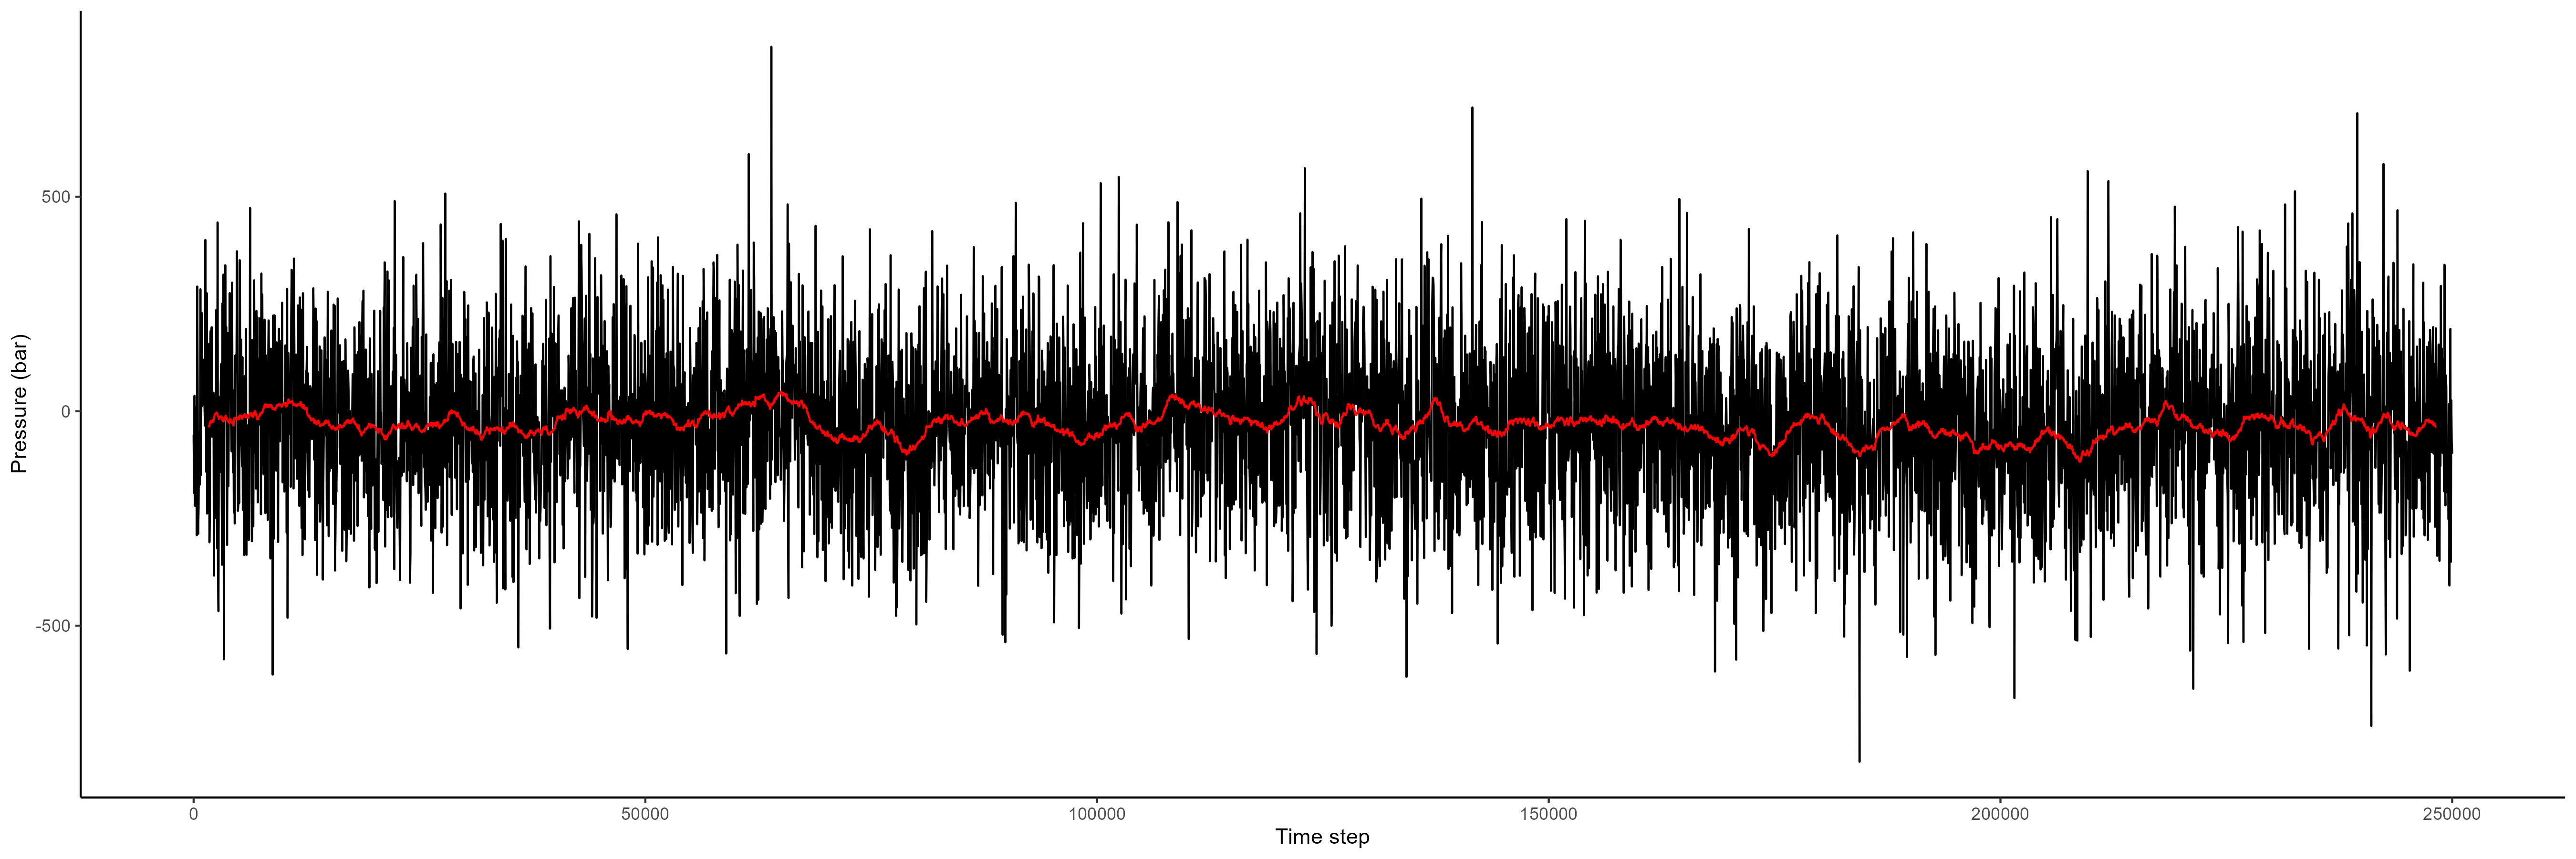
\includegraphics[width=0.8\textwidth]{Pressure_trace.png}
    \caption{Pressure vs. Time step. One time step is equivalent to 2 fs. The red line represents the moving average of the time series.}
    \label{pressure}
\end{figure}

The results for the RMSD, RMSF and pressure along the MD simulation showed an overall stability of the KcsA structure when is embedded in a lipid bilayer as POPC. These results led to evaluate the possibility that KcsA could be stable when is embedded in lipid bilayers of varying lipid compositions. Moreover, it is possible to think that similar proteins to KcsA could have a stable behavior as well, leading to possible studies on transmembrane proteins with similar characteristics.
\vspace{-5mm}
\bibliographystyle{ieeetr}
\bibliography{references}
\end{document}
